\documentclass[11pt]{article}
\usepackage[margin=0.5in]{geometry}
\linespread{1.15}
%\setlength{\parskip}{1ex}
%\setlength{\parindent}{0pt}
% \usepackage{parskip}
\usepackage{siunitx}
%\sisetup{group-separator={,},
%group-minimum-digits=6}
\usepackage{cofi}
\usepackage{fourier}
\usepackage{titling}
\usepackage[printwatermark]{xwatermark}
\newwatermark[allpages,color=black!20,angle=-55,scale=6,xpos=30,ypos=10]{DRAFT}



\setlength{\droptitle}{-0.6in}
\pretitle{\Large}
\title{MAT-150}
\posttitle{\hfill}
\preauthor{\hfill\Large}
\author{Project 1: Wind for Coal}
\postauthor{\hfill}
\predate{\hfill\Large}
\date{September 25, 2017}
\postdate{}

% Generated at 2017-09-20 15:59:52

% \NewDocumentCommand{\airDensity}{}{\num{1.2065}} %range 1.205 to 1.2075
% \NewDocumentCommand{\percentIncrease}{}{\num{24}} %range 22 to 26
% \NewDocumentCommand{\newLength}{}{\num{11}} %range 10 to 12
% \NewDocumentCommand{\oldLength}{}{\num{5}} %range 5 to 7
% \NewDocumentCommand{\mphWind}{}{\num{10}}  %range
% \NewDocumentCommand{\trialWatt}{}{\num{400}}

\usepackage{Sweave}
\begin{document}
\Sconcordance{concordance:P01_windturbine_original.tex:P01_windturbine_original.Rnw:%
1 14 1 1 7 1 16 21 1 1 0 9 1 1 15 223 1}

%\SweaveOpts{concordance=TRUE}

\thispagestyle{empty}
\maketitle
\thispagestyle{empty} \pagestyle{empty}




\subsection*{Project goals}
\vspace{-2.8ex}
\begin{compactitem}
    \item Practice modeling a real-world phenomenon that is not a routine
        homework exercise
    \item Become more comfortable with open-ended problems
    \item Practice communicating and explaining mathematical results clearly
        and professionally
    \item Practice working in a team on a mathematical problem
\end{compactitem}

\subsection*{Project synopsis}
\vspace{-2.8ex}

\begin{minipage}[t][2.6in]{0.65\textwidth}
    \vspace{0pt}

    You and your group members are mathematical consultants working on a
    project to determine whether electric power generated by wind turbines
    could replace the electricity generated by a coal plant that Idaho Power
    is planning to shut down, at North Valmy Generating Station in Nevada. Its
    254-megawatt Unit 1 plans to go
    out of service in 2022, while Unit 2, rated at 268 megawatts, will go out of
    service in 2025. A group of investors have hired your group to explore
    whether the power generated by Unit 1 could be replaced using
    wind turbines in eastern Idaho. They have an innovative design for an
    efficient turbine, but before investing more money in development, they
    want to know if the project is worth pursuing. The major costs to the
    project depend on the number of turbines required to replace the
    electricity generated by Unit 1 and the number of acres of land
    the investors will need to acquire for the turbines.

    %Your group is tasked with estimating the number of turbines and how much
    %land will be needed. Your report should also include a recommendation on
    %whether or not to proceed with the project based on your findings.

    % \vspace{1.18ex}


    \end{minipage} \hspace{1em}
    \begin{minipage}[t][2.6in]{0.32\textwidth}
        \vspace{0pt}
    % \begin{figure}[h]
    %    \centering

       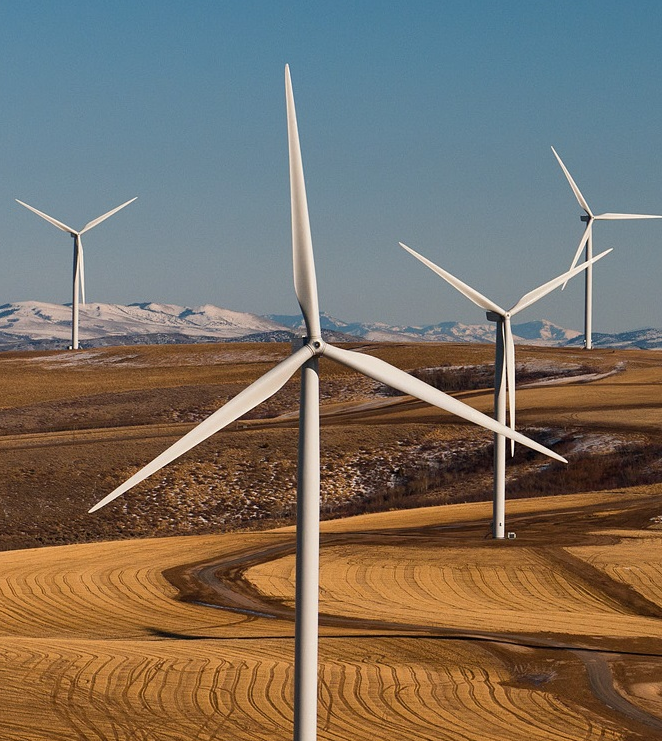
\includegraphics[width=\linewidth, keepaspectratio=.8]{windturbines.png}
    % \end{figure}
    \end{minipage}

\subsection*{Useful facts and assumptions}
\vspace{-2.8ex}

    \begin{compactitem}

        \item Your sense is that dimensional analysis might help in
        determining an expression for the generated power $P$ in terms of the
        wind velocity $v$. Some other important quantities are the length $L$ of the
        turbine blades and the ambient density of the air $\delta$. In
        general, $\delta$ varies with altitude and humidity, but for this
        report, assume $\delta = \SI{1.207}{kg/m^3}$. Other
        effects can be ignored.
        \item You remember that an expression arising from dimensional
        analysis will have an unknown constant of proportionality in it, which
        you hope to estimate from the data you have. This dimensionless
        constant depends primarily on the shape of the turbine blades.
        \item The investor's engineers believe with their design for a more
        efficient turbine will increase the power generated by 
        24\% over their trial turbine which was built and
        tested two years ago.
        \item The trial turbine has a blade length of approximately
        $\SI{5}{ft}$, and generates
        $\SI{12000}{W}$ of power in winds of
        $\SI{11}{mph}$.
        \item The group plans a turbine larger than the trial model. They plan
        to use a blade length of $\SI{10}{ft}$.
        \item While wind speeds in Idaho Falls average about
        $\SI{4.6}{mph}$, the maximum speed each day averages
        about $\SI{11}{mph}$. We expect conditions at the farm
        to be slightly windier, but this is the data we have.
        \item For best efficiency, the engineers want the turbines to be
        spaced at least $3$ blade lengths apart, measured from the center of
        the turbine's tower.

    \end{compactitem}

% \newpage

    Your team must now pull together all of its ideas to calculate an estimate
    of the power generated by the proposed new turbine, determine the number
    of turbines needed to replace the power from North Valmy's Unit
    1 and estimate the number of acres of land the investors would
    need to acquire for this project. Once you finish your calculations, write
    a professional report summarizing your work and your findings to the
    investors. Include a recommendation as to whether your group considers the
    project worth pursuing. Be sure to justify your recommendation. You should
    report your answers with two significant digits.

    %Note that not all of the investors are engineers or mathematicians and
    %your report must clearly explain your methods so that all of the
    %investors understand your analysis. A carefully labeled graph, created in
    %R, should be included in your report to support your recommendation.

 %\newpage

\subsection*{Report guidelines}
\vspace{-2.8ex}


\begin{compactdesc}
    \item[Preliminary check-in:] Thursday/Friday, October 5--6, with your
    instructor at a scheduled time.
    \item[Final report due:] Wednesday, October 11, by the beginning of
    class, in Canvas.
    \item[Group evaluations due:] Wednesday, October 11, by 11:59pm, in
    Canvas.
    \item[Final interview:] Thursday/Friday, October 12--13, with your
    instructor at a scheduled time.
    \item[Late papers/group evaluations/missed interviews:] will not be accepted.
\end{compactdesc}

\subsection*{Preliminary check-in and final interview meetings}
\vspace{-2.8ex}

Your group turns in one report which will be submitted through Canvas.
Everyone in the group gets the same grade for the Written Report section for
this project. The Written Report accounts for $35\%$ of your Project 1 grade.
The rest of your score ($65\%$) is earned during the Preliminary Check-in
($25\%$) and Final Interview ($25\%$) meetings with your instructor. In these
meetings, you will answer a question regarding the development of the report's
results to demonstrate your participation in the project. You are expected to
participate in the project, understanding both the solution to the problem and
the process by which it was obtained. Your group will bring a printout of the
Introduction to your report to the Preliminary interview ($10\%$) and each
member of the group will submit a group evaluation ($5\%$) at the end of the
project. Your group evaluation will not effect the grade of any of your group
members.

\subsection*{Written report}
\vspace{-2.8ex}

Use Microsoft Word or another suitable word processor. \textbf{Type all
equations}, using (for example) the Microsoft Equation Editor built into Word
and standard mathematical notation. Use RStudio to make all graphs. Graphs
must include proper axis labels. Group members' names and class section (01 or
02) must be clearly visible on the front page of your report. Margins will not
exceed 1 inch and lines are to be no more than 1.5-spaced. Use a font such as
Calibri or Times New Roman with a font size of 12 points.

Reports will be self-contained, i.e., the reader will not need prior knowledge
or understanding of the problem to understand your report. Your calculations
and conclusions will be explained in detail, as befits a professional report.
This report will be used by people of varying mathematical background, so do
your best to keep your report at a level accessible to the widest possible
audience (in other words, try to write for the general public whenever
possible). Your explanation and presentation are as important as the
mathematics, but of course your mathematical analysis must be clear, complete,
and correct. It should go without saying that your grammar, punctuation, and
spelling will be flawless.

\subsection*{Group evaluation}
\vspace{-2.8ex}

Every group member is required to submit to their instructor an informal group
evaluation \emph{the same day the reports are due}. The evaluation is at most
a short paragraph about how well the group worked together. The evaluation
\emph{must} include your estimate of the share of the project work that you
feel each group member did, expressed as a percentage (e.g.~33\%/33\%/33\% or
40\%/30\%/30\%, etc.). These percentages must add to 100\%---or 99\% is close
enough. These evaluations will be held in confidence, and used at the end of
the semester, if necessary, to adjust final grades.

\subsection*{A word to the wise}
\vspace{-2.8ex}

This project counts for 10\% of your final grade. Please make sure that
your report's qualities of clarity, completeness, and correctness
reflect your best abilities. Please carefully read all the instructions
and resources provided. \hfill Group ID: 56a50ed7

%%%%%%%%%%%% BEGIN ANSWER KEY SECTION %%%%%%%%%%%%%%

\newpage

\section*{Key for group 56a50ed7}

For the trial turbine:

\begin{compactenum}
    \item $L = \SI{5}{ft}$
    \item $v = \SI{11}{mph}$
    \item initial power $P = \SI{12000}{W}$
    \item percent increase = $0.24$
    \item increased power $P = \SI{14880}{W}$
    \item proportionality constant (dimensionless) $k = 0.0446383895970886$
    \item proportionality constant (dimensionful) $k = 0.370490944073421$
\end{compactenum}

For the new turbine:

\begin{compactenum}
    \item $L = \SI{10}{ft}$
    \item $v = \SI{14880}{W}$
    \item $P = \SI{4352.69625845229}{W}$
    \item $P = \SI{4352.69625845229}{W}$ (computed with dimensionful $k$)
\end{compactenum}

Put it all together:

\begin{compactenum}
    \item Unit $1$ needs \SI{254}{MW}
    \item This requires $58354.6346719622$ turbines
    \item Each turbine needs about $\SI{1089}{ft^2}$
    \item There are $43560$ square feet in an acre
    \item So we will need $1458.86586679905$ acres
\end{compactenum}

%%%%%%%%%%%% END ANSWER KEY SECTION %%%%%%%%%%%%%%

\end{document}
